\chapter{Foundations and Technical Background}
\label{chap:foundations}
%\index{TF$\cdot$IDF}
%\index{TF|see{TF$\cdot$IDF}}
%\index{IDF|see{TF$\cdot$IDF}}
%\index{DF|see{TF$\cdot$IDF}}
%\index{Keyword Query}
%\index{Okapi BM25}
%\index{Keyword Query}
%\index{Phrase Query}
%\index{Proximity}
%\index{Query Processing!Term-at-a-Time}
%\index{Term-at-a-Time|see{Query Processing}}
%\index{Query Processing!Document-at-a-Time}
%\index{Document-at-a-Time|\\see{Query Processing}}
%\index{Query Processing!Early-Terminating Methods}
%\index{Query Processing!NRA}
%\index{NRA|see{Query Processing}}
%\index{Index Updates}
%\index{Update Algorithms}


In this chapter, we introduce the technical background necessary to understanding the contributions presented in this thesis. We start with a brief description of web archives and recent efforts relating to their acquisition and preservation. Next, we give an overvi\-ew of information retrieval with focus on text retrieval. In particular, we focus on the efficiency aspects of text retrieval and describe issues concerning indexing and query processing over large text collections. Finally, we conclude with the state-of-art techniques relating to indexing archives.


\section{Web Archiving} 
%\index{Internet Archive}
%\index{IIPC}
%\index{European Archive}

  \begin{figure}[tb]
  \centering
    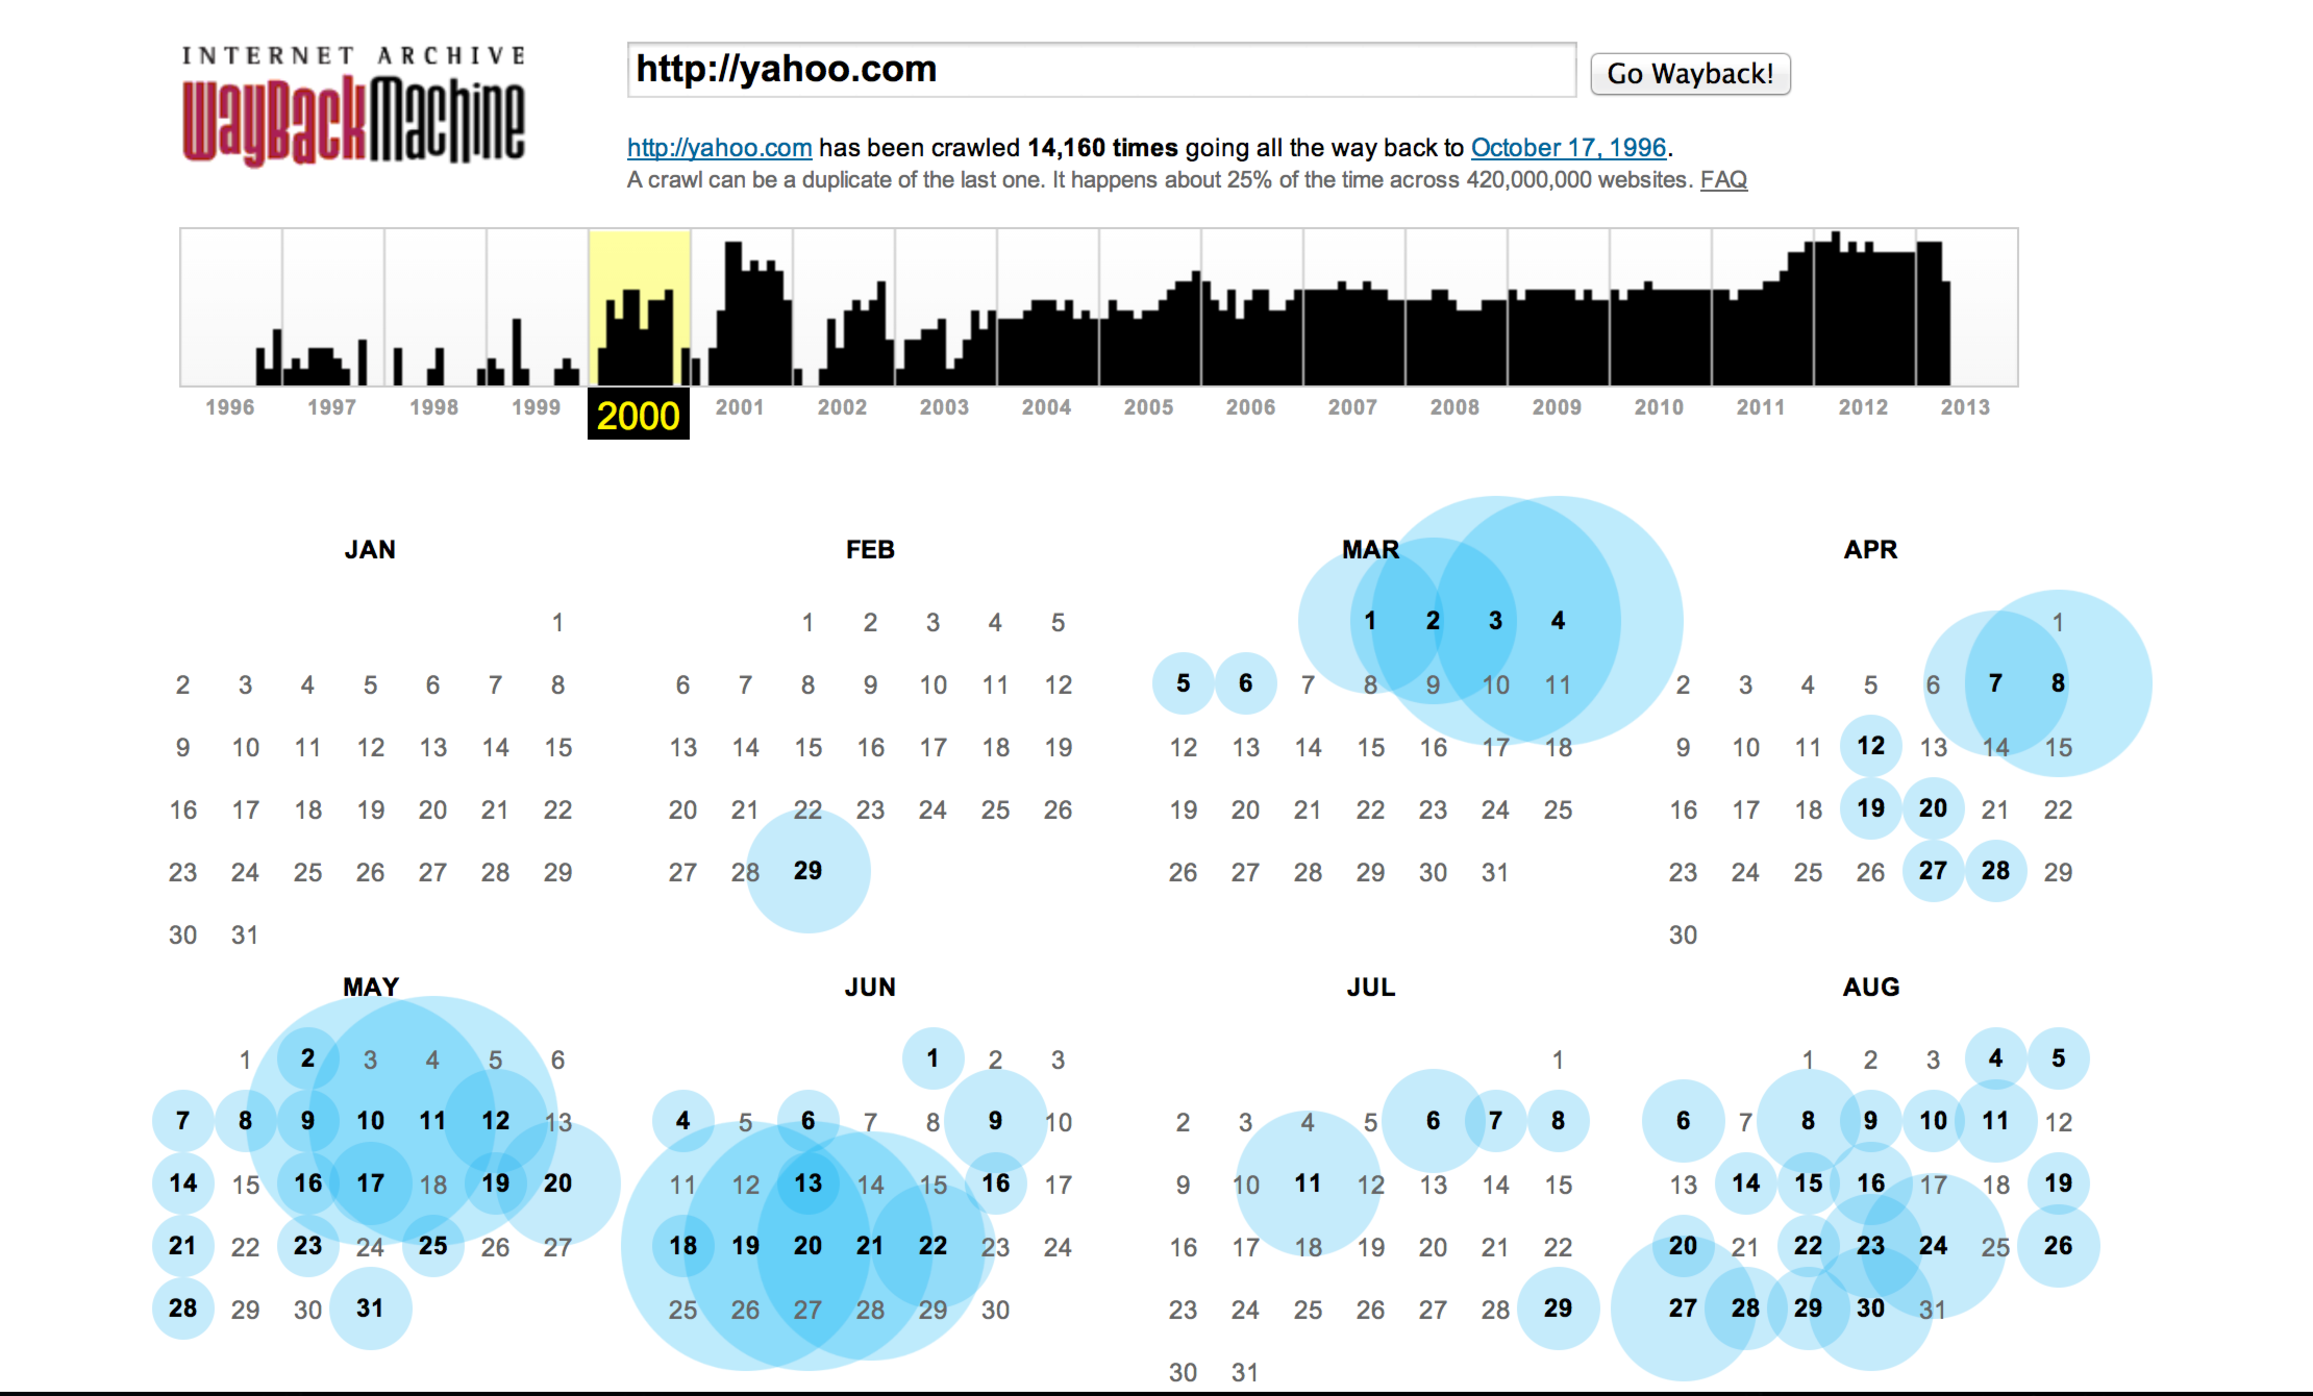
\includegraphics[width=\columnwidth]{resources/wayback_machine.pdf}
  \caption{Website preserved by \emph{Internet Archive}} 
    \label{fig:ia_example}
\end{figure}


The Web is in a continuous state of change~\cite{1498837,Cho, 775246}. Existing pages are modified, new content is added, and old pages are removed resulting in a change of state of the Web. Web archives prevent this loss by attempting to capture and preserve this knowledge before it disappears. Efforts to preserve web contents have been undertaken both by governments~\cite{webarchive,netarkivet,bnf,pandora}, non-profit organizations~\cite{IA, IM}, and companies~\cite{HANZO}. Undoubtedly, the most popular and large-scale effort in archiving the web has been the \emph{Internet Archive}~\cite{IA} which has an estimated size of 500 Terabytes and is growing at 100 Terabytes a year. 


\paragraph{Crawling in Web Archives} Crawling is the most common method of acquiring content for web archives. A web crawler systematically requests and stores content from web pages. It starts visiting pages from a seed set of pages and traverses the website in a breadth-first or depth-first manner. The key difference from crawling strategies in standard web search is that all files require to be fetched as opposed to only the ones which would be later indexed. The challenges in crawling for archiving is usually in capturing a consistent snapshot of a website at a given instance. Usually, due to politeness requirements, it takes a long time to crawl an entire website. In the meanwhile many portions of the website might undergo changes and modifications which are not captured. Figure~\ref{fig:ia_example} shows how often and when \texttt{yahoo.com} has been crawled and preserved by the Internet Archive.

Denev et al.~\cite{denev2011sharc} propose a model for assessing the quality of the crawled data for web archives. They define \emph{blur} as a stochastic measure of the quality of capture. The longer it takes to capture an entire website the more blur the gathered data is said to have. Further, \emph{coherence} is a deterministic quality measure which determines the accuracy of a snapshot, i.e., number of pages which did not change during the crawl. They further propose effective crawling techniques which optimize for blur and coherence. 

The Internet Preservation Consortium (IIPC)~\cite{IIPC} and other preservation organization are involved in establishing standards necessary for effective web preservation. IIPC is also involved in the development of open source software, most prominently Heritrix~\cite{digitalHistory:www}, for crawling for web archives. For other issues and best practices in web archives please refer to~\cite{masanes2006web}. 

Although there has been progress in content acquisition for web archives; access methods and search support over them have been limited. Most of the archives either do not have an explicit search interface or provide limited search functionality based on open-source tools like Nutch~\cite{nutchwax} or Solr~\cite{solr}. 

%\paragraph{Prevalent ways of accessing, exploring and searching archives}

\section{Data Management}
In this section we look at various data management principles and techniques which are either related or used in our work. We briefly discuss the work done in temporal databases which also deals with managing temporal data. Next, we give a detailed account of distinct value estimators and KMV synopsis which we require in Chapter~\ref{chap:selection} in our work on query optimization for time-travel text search.

\subsection{Temporal Databases}

Temporal databases deal with data management issues pertaining to data associated with temporal aspects. Specifically these temporal aspects include the notion of \emph{transaction} and \emph{valid times}. Transaction time refers to the time when a certain fact was stored in the database. Valid time, on the other hand, refers to the time when the fact existed or was active in the real world. As an example if we enter a fact about the great depression of 1930's into the database, the valid time would refer to a time-interval [1930 - 1940], while the transaction time would be when the entry was made, for example March 2013. Transaction times evolve linearly and are immutable to change in the past unlike valid times where changes in the past are allowed. Research in temporal databases has proposed models, query languages and indexing techniques over arbitrary data with such temporal aspects. 

%However, we deal specifically with text with a temporal model resembling transaction times. \aanand{reformulate..}

We now discuss in brief about notable index structures and indexing methods for transaction time data. Early approaches, like the Time-Split B-trees (TSBT)~\cite{lomet1993exploiting} and Multi-Version B-trees (MVBT)~\cite{becker1996asymptotically}, adapt B$^+$-trees for time-evolving data. The Time-Split B-Tree was aimed at reducing storage costs and improving query performance over current records but did not provide good worst case guarantees. MVBT overcame this problem and also provided the same asymptotic space and time complexity as the B-tree when a single version per record is managed. 

In the late nineties, the \emph{log-structured history data access method} (LHAM) was proposed by Muth et al.~\cite{Muth2000} for data with high update rates. LHAM stores its data in successive components $C_0,\ldots,C_m$ of varying sizes and access costs. The core idea is that the most recent data is stored in the component with the least access cost $C_0$ thereby improving update performance. The older records are gradually merged into components with high access costs $C_{i+1}$ whenever a component $C_i$ is full. The partitioning of records into components entails a partitioning of the entire time duration into non-overlapping time intervals. Consequently, each component $C_i$ is associated with a time interval. Typically the component sizes follow a geometric progression and whenever a $C_i$ is full it potentially triggers a series of merges via a \emph{rolling merge} operation. A detailed survey of access methods for temporal databases can be found in~\cite{salzberg:csur1999}.

\subsection{Synopsis Structures}

Determining number of distinct values in large collections, termed as \emph{distinct-value estimation} or \emph{DV estimation}, is an important task in query optimization, data streams and network monitoring. While the exact count of distinct values is desired, determining them is both computationally expensive and does not scale well. To this extent, approximate methods have been proposed in the literature which efficiently estimate the result like Bloom filters~\cite{bloom1970space}, Hash Sketches~\cite{flajolet1985probabilistic} and KMV Synopsis~\cite{kmv:sigmod}. These approaches are based on concise data-structures constructed over the input called \emph{synopsis} or \emph{sketches}. In this section we give brief background information on the synopsis structures, and specifically KMV synopsis, that are utilized by our algorithms.

\subsubsection{Bloom Filters}
It is a space-efficient probabilistic data structure used for answering set membership, set containment, or set-intersection queries with a high confidence. Bloom filters are concerned with sets and offer less than 10 bits per element for a 1\% false positive probability. However, they cannot be employed for arbitrary multiset operations.

\subsubsection{Hash Sketches}

These are distinct-value estimation technique was proposed in~\cite{flajolet1985probabilistic}. They rely on a pseudo-uniform hash function over the input to derive a sketch. These sketches allow for various multiset operations by counting distinct elements after allowing appropriately combining the sketches. Multiple intersections introduce high relative errors and has a high computational complexity.


\subsubsection{KMV Synopsis} 
Beyer et al.~\cite{kmv:sigmod} introduced \textit{KMV synopses} 
as effective sketches for sets that support arbitrary multiset operations including union, intersection, and differences. They differ from hash sketches in having lower computational costs and more accurate DV estimation. In this section we first explain the principle of DV estimation and introduce the KMV synopsis data structure. We then explain how multiset operations like \emph{union, intersection} and \emph{set difference} can be applied to them and estimated.

Consider an input multiset $S$ with $D$ distinct values $\Theta(S) = \{v_1,v_2, \dots,v_D\}$ where $\Theta(S)$ represents the domain. Each of these values is mapped to a random location on an unit interval. Assuming that the points are distributed uniformly, the expected distance between any two neighboring points is $1/(D+1) \approx 1/D$. The expected position of the $k$-th point from the origin or the $k$-th smallest point, $U_{k}$, , is $k/D$, i.e, $E[U_{k}] \approx k/D$. The simplest estimator of $E[U_k]$ is simply $U_k$ and yields the \emph{basic estimator} as introduced in~\cite{bar2002counting}:

\begin{equation*}
\label{eq:basicestimator}
\hat{D}^{BE}_{k}=k  / U_{k}.
\end{equation*}
 
 Consider a hash function $h: \Theta(S) \mapsto {0,1, \dots,M}$ which maps the input in the range $[0-M]$ where $M >> D$. The hash function $h$ is chosen such that mapped values $h(v_1),h(v_2), \dots,h(v_D)$ resemble an independent and identically distributed sample from the discrete uniform distribution on ${0,1, \dots,M}$. Normalizing the range to a unit range, as above, the values $U_i$ can be expressed as $U_i = h(v_i)/M, v_i \in \Theta(S)$. The value $M$ regulates the number of collisions. The higher the value of $M$ the lower the probability of collisions.

Building on this notion of the basic estimator, KMV synopsis is defined in~\cite{kmv:sigmod} for a multiset $S$ as follows. Given a hash function $h$, the $k$-smallest values of the mapping $h(v_i)$ where $v_i \in \Theta(S)$ constitute the KMV (k-minimum values) synopsis of $S$. Typically $M = \mathcal{O}(D^2)$ is chosen to avoid collisions and hence each of the synopsis values can be encoded in $\mathcal{O}(\log{D})$ bits. Consequently, the number of bits required to store the KMV synopsis is $k\, \mathcal{O}(\log{D})$. The KMV synopsis can be created by a single scan over $S$ and only storing the $k$ smallest hashed values implemented efficiently by a priority queue. The basic estimator is further extended to an unbiased estimator $\hat{D}_{k}$.

\begin{equation*}
\label{eq:kmvestimator}
\hat{D}_{k}=(k-1) / U_{k}
\end{equation*}

The cardinality estimation of the multiset operations involving two or more synopses, like unions and intersections, can be carried out efficiently based on the above estimators. 


\section{Information Retrieval}
\label{sec:ir}

Information retrieval (IR) deals with finding information from large collections of unstructured data to satisfy user information needs. Historically, the focus of IR has been on investigating concepts, models and computational methods for searching large text collections. However, the field has expanded its horizons to multimedia content~\cite{chowdhury2010introduction}, facts and semi-structured content~\cite{lalmas201225, croft2010search}. In this work we focus on text collections and deal with the core problem in IR, i.e.,

\emph{We are given a document collection $\mathcal{D}$ associated with a vocabulary of terms $\mathcal{V}$. For a given query $q\in \mathcal{V}$ our aim is to find the documents which satisfy the user information need expressed by $q$.} 

% \emph{Given a document collection $\mathcal{D}$ of documents $d \in \mathcal{D}$, associated with a vocabulary $\mathcal{V}$ of terms $v \in \mathcal{V}$, we intend to find the documents which satisfy the user information need expressed by a query $q$, $q \in \mathcal{V}$.} 

%The collection $\mathcal{D}$ is associated with a vocabulary $\mathcal{V}$ of terms $v \in \mathcal{V}$ which are constituents of documents and queries. 

\subsection{Retrieval Models}
%\index{TF$\cdot$IDF}
%\index{TF|see{TF$\cdot$IDF}}
%\index{IDF|see{TF$\cdot$IDF}}
%\index{DF|see{TF$\cdot$IDF}}
%\index{Keyword Query}
%\index{Okapi BM25}
%\index{Boolean Retrieval}
%\index{Boolean Query}
%\index{Vector Space Model}
%\index{Keyword Query}


The question above gives rise to two key aspects which account for the \emph{effectiveness} of IR systems -- (1) How are documents and queries modelled ? (2) How is the relevance of a document to a given query modelled ?

\paragraph{Boolean Retrieval} Many retrieval models have been proposed to model documents and queries and the similarity between them. We provide the key ideas of some of the fundamental retrieval models. The \emph{Boolean retrieval model} is the earliest and simplest retrieval model. Queries in this retrieval model are Boolean expressions comprising of terms $v \in \mathcal{V}$ and connected by Boolean operators (\textsc{or, and, not}). The notion of relevance of a document $d$ to a query $q$ is binary, i.e., either $d$ is relevant to $q$ or not depending on the evaluation result of the Boolean expression. 

\paragraph{Ranked Retrieval} Salton introduced the \emph{vector space model}~\cite{salton1975vector} to rank documents according to their perceived relevance to the query by modelling documents and the query as a vector of features. The features are typically \emph{terms} in this case and the similarity value between a query and a document encodes the relevance of a document given a query. The similarity between $q$ and $d$ is given by the \emph{cosine similarity} between the document and query vector cast in the feature space of terms. 

\paragraph{Query Semantics} There are two widely accepted query semantics -- \emph{conjunctive} and \emph{disjunctive} query semantics. Conjunctive query semantics require all terms to be present in a document to qualify as a relevant result whereas disjunctive semantics allow any occurrence of the query terms in the document. For example, under conjunctive query semantics, the relevant documents for the keyword query \kwquery{german soccer team} using boolean retrieval should contain all the constituent terms \kwquery{german}, \kwquery{soccer} and \kwquery{team} to constitute as results. Although simple to implement, Boolean-retrieval models are limiting when a large number of documents qualify as results. It is hard for the user to evaluate all results and a notion of ranking is hence desirable.

We now come to the question of assigning feature values for vectors. To address this there are two aspects which are considered. The more a query term occurs in a document the more important it is. This is captured by the term frequency or $tf(d,v)$ of a term $v$ for a document $d$, which is defined as the number of times $v$ is present in $d$. Note that in this model, documents are considered as \emph{bags} of terms. However, certain terms frequently occur throughout the corpus, for instance articles, prepositions and stop words. These terms, although highly frequent, might not be \emph{discriminative} from other query terms when it comes to capturing the true user intent. For example in the query \kwquery{house of fraser}, \kwquery{fraser} is more discriminative than the other terms which appear frequently in the collection. To account for this, the second aspect or document frequency $df(v)$ of a term $v$ is taken into consideration. Using the value $df$, the inverse document frequency is defined as 
$$ idf(v) =  \log \frac{|\mathcal{D}|}{df(v)}$$
is construed as being directly correlated with the discriminativeness of a term.

Combining both the measures we arrive at the $tf$-$idf$ which has become one of the most central weighting scheme for the vector space model. Most of the other weighting schemes are often variations and refinements of $tf$-$idf$. A detailed account of these weighting schemes can be found in Manning et al.~\cite{Manning:2008fk}. The most popular refinement of the $tf$-$idf$ value is the Okapi BM25 model by Robertson et al. which is known to provide high retrieval effectiveness. Okapi BM25 takes into account the length of the document and also the average length of documents in the entire collection to normalize the term frequencies. Formally,

\begin{definition}[Okapi BM25]
For a document $d$ and a query $q$, the relevance of $d$ to $q$   is defined by Okapi BM25 as

\begin{equation}
	r(q,d) = \sum_{v \in q} w_{tf}(v, d).w_{idf}(v). 
\end{equation}

The $tf$-score $w_{tf}(v, d)$ is defined as
  \begin{equation}
    \label{eq:5-ttix}
    w_{tf}(q, d) = \frac {(k_1 + 1) \cdot tf(q,d)} {k_1
      \cdot ((1-b) + b \cdot \frac{dl(d)}{avdl}) +
      tf(q,d)}\;,
  \end{equation}
where $0 \leq b \leq 1$ and $k_1 \geq 1$ are tunable parameters. The length of $d$ is denoted as $|d|$ and $avdl$ represents the average document length in the document collection. 
$$
$$
The $idf$-score is defined as
 \begin{equation}
    \label{eq:5-ttix}
    w_{idf}(v) = \log{\frac{N - df(v) + 0.5}{df(v) + 0.5}}\;,
  \end{equation}
where $N$ is the collection size and $df(v)$ has the aforementioned semantics.
\end{definition}

The $tf$ component in Okapi BM25 is scaled by adjusting the parameter $k_1$ while $b$ controls the effect of length normalization. Typical values for the two parameters which have been seen to work well are $k_1 = 1.2$ and $b=0.75$.


The success of a retrieval system not only depends on the effectiveness of the retrieval models but also on how fast it can respond to queries. With the exponential growth of collection sizes the challenges for scalable and efficient search have accounted for a rich body of research over the past decade. The efficiency issues can be broadly classified into two major areas in the retrieval phases -- (i) indexing the document collection and (ii) processing queries over the index. In the following, we introduce the common techniques employed for indexing text. 

\subsection{Indexing Text}

 \begin{figure}[tb]
  \centering
    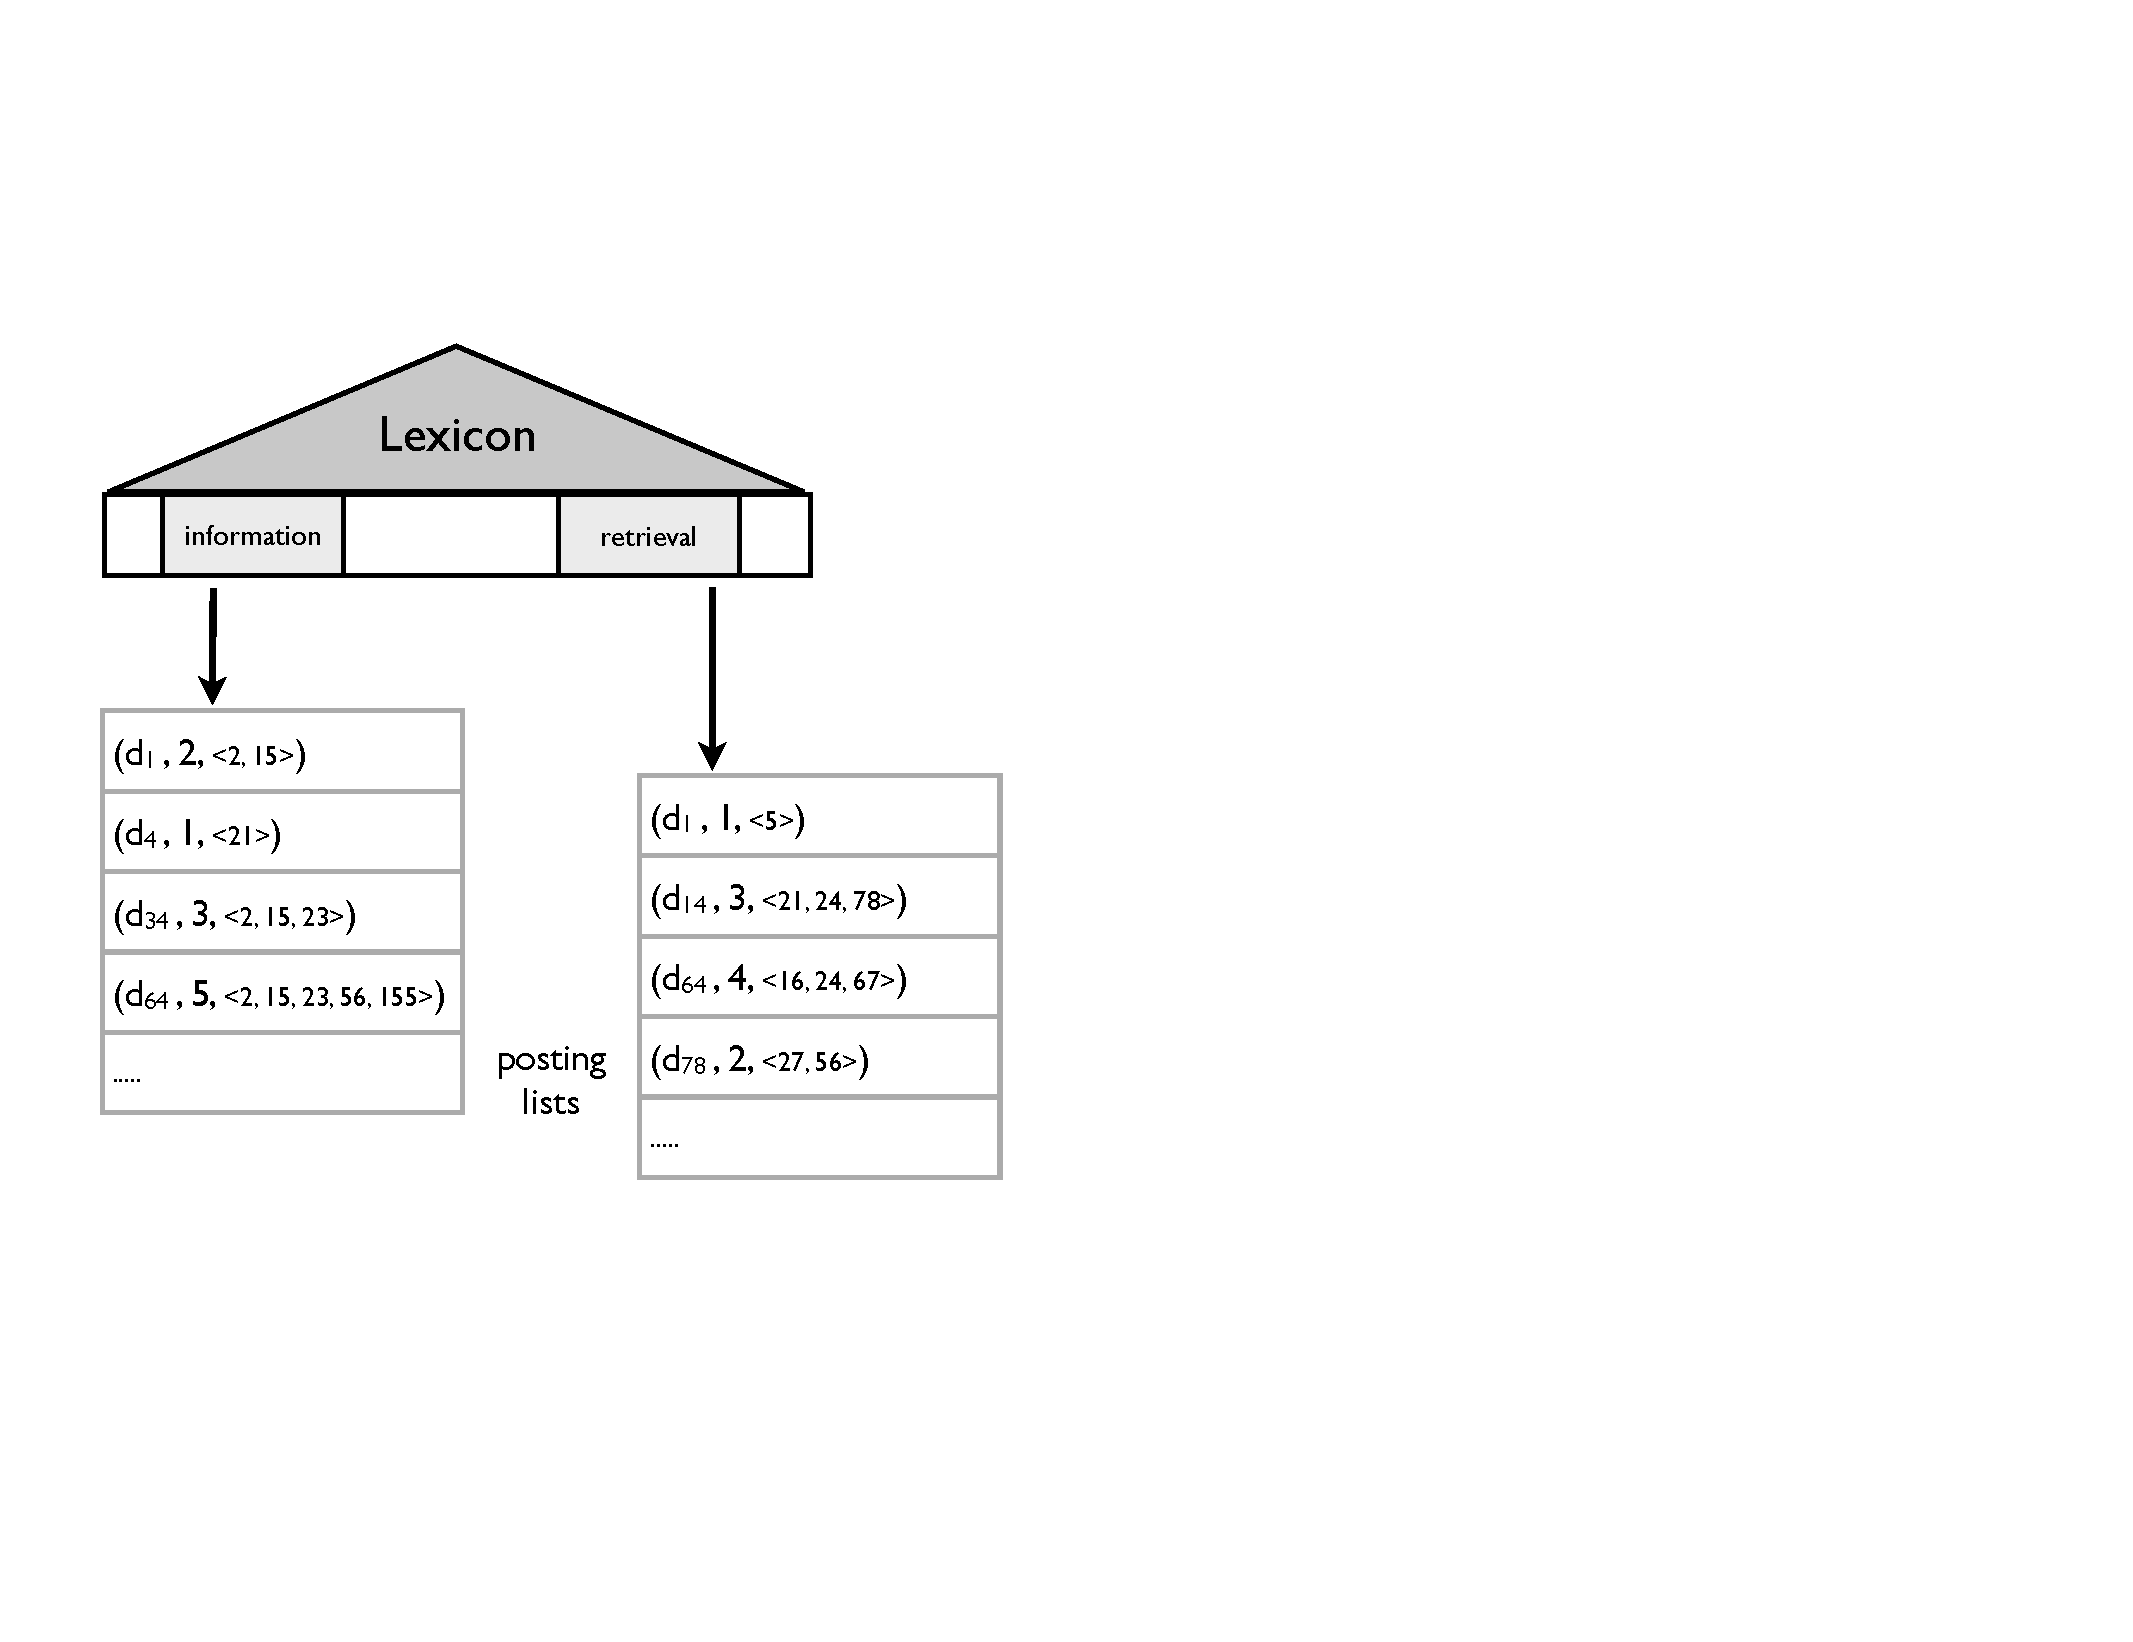
\includegraphics[width=0.6\columnwidth]{resources/inverted_index.pdf}
  \caption{Inverted index} 
    \label{fig:inverted_index}
\end{figure}


Indexing methods are required in order to efficiently perform the retrieval process. The most popular choice to index text collections is the \emph{inverted index}. It is the cornerstone for most commercial search engines and real-world information retrieval systems.  The inverted index comprises of two components - (i) the \emph{lexicon} and the (ii) collection of \emph{posting lists} comprising the \emph{inverted file}. Each of them can be implemented using different data structures and are materialized into separate files.

\paragraph{Lexicon} The lexicon or the term dictionary contains the indexed terms and their corresponding statistics. These terms are 
typically words which are extracted and stemmed from individual documents. Each entry in the lexicon represents a term $v$ and it must contain, but is not limited to, the following -- (i) the string of the term $v$, (ii) document-frequency information $df(v)$ and, (iii) pointer to the posting list of $v$ in the postings file. 

During query processing the lexicon is consulted to check for the containment of the query terms in the collection. The look-up process results in providing further data, if needed, for the rest of the retrieval process. There are many strategies to improve lexicon look-up speeds. One straightforward approach, which is now common with the growth of memory capacities, is to load the entire lexicon into memory as a hash table. Other examples of dictionary layout include search trees and \emph{dictionary-as-a-string} proposed by Witten et. al~\cite{Witten:1999fk}. For a detailed discussion we point the reader to Manning et al.~\cite{Manning:2008fk}.

\paragraph{Postings File} 

The second data structure is the postings file which contains information about occurrence of terms in documents. Since terms are the indexed units here, each term $v$ is associated with a list of postings $L_v$, called the \emph{posting list}, and each posting represents a document where $v$ is present. The postings file is a collection of posting lists, one for each term. A posting belonging to the posting list $L_v$, contains the document identifier $d_i$ where $v$ is present and information about the $v$'s occurrences. The occurrence information can be binary, if $v$ is present in the document or not, or more expressive, like the frequency of occurrences or even positions where $v$ was present in the document, i.e.,
$$
	\langle d_i,\,\, tf(v,d_i), \,\, <pos_1, \ldots, pos_{tf(v, d_i)}> \rangle.
$$

For Boolean retrieval storing only document identifiers is sufficient. In case of ranked retrieval, which is indeed the more common scenario, a score $s$ is stored which is usually the $tf(v,d_i)$ or $tf(v,d_i).idf(v)$. If phrase or proximity queries need to be supported the posting also stores a list of positions where the term occurs in the document (see Figure~\ref{fig:inverted_index}). These positions are sorted for best compression and query processing benefits as we will see later. Posting lists are highly compressed and stored contiguously on disk for best space and cache effectiveness. However, for dynamic collections the contiguous placement might not always be desirable and we discuss later how such collections can be indexed. Additionally these lists can be augmented with \emph{skip pointers} for faster list traversal during query processing~\cite{DBLP:journals/tois/MoffatZ96}. For the scope of this work we do not consider such optimizations, since they are orthogonal to the methods proposed.

The posting list can be \emph{document-ordered} or \emph{score-ordered}. In document-ordering the postings are ordered by increasing document identifiers. The benefit of such an organization is that it achieves high compression ratios. Additionally, document-ordered lists are easier to maintain than their score ordered counterparts. On the other hand score-ordered lists are ordered according to their scores. Score-ordered lists facilitate dynamic pruning of lists during query processing and do not require the entire list to be read into memory. Several top-k algorithms have been proposed which allow for early termination by leveraging the score order during query processing~\cite{arai2007anytime, fagin2001optimal, bast2006io, theobald2004top,yuan2012efficient}. However, the compression factor achieved by such an ordering is not as high as document-ordered lists and index maintainance is also expensive.

\subsubsection{Compression}

The posting list accounts for the majority of the index size. Thus posting-list compression is a key problem in indexing text and has been subject to active research over the past two decades. The obvious advantage of list compression is their savings in overall index size. Since inverted indexes are typically stored on disk, compression can reduce the space consumption by 75\%~\cite{Manning:2008fk}. Also, due to the use of caching for query processing, some of the frequently accessed index lists are stored in memory to increase query performance. Since, memory is a more expensive resource than disks, a smaller memory footprint is desirable. 
%Finally, improvements in the processing power of CPUs have been faster relative to the growth in performance of hard disks. 
Finally, CPU performance has improved relatively more than hard-disk performance in recent years. Thus the aggregate benefit of transferring a highly compressed posting list to memory and decompressing it outperforms reading it in its uncompressed form. We outline the most widely used techniques for index compression. 

\paragraph{Integer Compression} We first talk about integer-compression techniques useful in compressing document identifiers and positional information. Storing integers in fixed-size bit sequences or arrays wastes space for small integers. 
\emph{Variable byte encoding} uses integral number of bytes to encode an integer. An example is the \emph{7-bit encoding} in which the most-significant bit of a byte is the \emph{continuation bit} and the remaining seven bits represent the payload. The 7-bit encoding can be decoded by reading a sequence of bytes until the continuation bit is zero. The sequence read concatenates the payloads of each byte, disregarding the continuous bit values of each byte, to decode the integer. As an example, $n = 129$ is encoded as $\seq{00000001 \,\,\,\, 11111111}$ and $n = 30$ is $\seq{00011110}$. 


Unlike variable byte encoding, which is byte aligned, we can consider directly working with bits. The simplest bit-level encoding technique \emph{unary encoding} stores $n-1$ one bits followed by a zero as a delimiter to store the positive integer $n$. Although, it is beneficial for small $n$ it soon becomes infeasible for higher values of $n$. For more efficient representations of integers \emph{Elias}-$\gamma$ \emph{encoding} is used which splits the positive integer $n$ into two parts. The first part encodes $1 + \lfloor \log{n} \rfloor$ in unary encoding. The second part encodes $n - 2^{\lfloor \log{n} \rfloor}$ using binary encoding. As an example $n=10$ would be encoded as $\seq{1110 \,\,\,\, 10}.$

\emph{Elias}-$\delta$ \emph{encoding} is slightly different from \emph{Elias}-$\gamma$ \emph{encoding} in which the first part, $1 + \lfloor \log{n} \rfloor$, is encoded using \emph{Elias}-$\gamma$ \emph{encoding} instead of unary encoding. Thus, $n=10$ would now be encoded as $\seq{110 \,\,\,\, 00 \,\,\,\, 10}.$

\paragraph{Compressing d-gaps} Let us for simplicity view a posting list as an array of document identifiers. The obvious choice in compressing a posting list is to use one of the above techniques to compress each document identifier $did$. In case of document-ordered lists, we can exploit the ascending order of $did$s by encoding the difference between consecutive $did$ values or so called \emph{d-gaps}. In this scheme, the original integer value of only the first or minimum integer is stored. The remaining integers are represented by their d-gap value. All integers can be reconstructed in the course of the linear scan from begin of the list from the d-gaps. For example $\seq{d_1,d_2,d_2,d_4}$ can be represented as $\seq{d_1\,,d_2-d_1\,,d_3 - d_2\,,d_4-d_3}.$

The primary advantage of storing d-gaps is that they tend to be small integers and can be compactly represented using the techniques discussed above. The gains are significant especially for long posting lists, corresponding to frequent terms such as articles or preposition, where the difference between $did$s is very small. Apart from using d-gaps for $did$s it can also be employed for positional information. A more comprehensive survey of other compression methods for d-gaps can be found in~\cite{Witten:1999fk}. 

\subsubsection{Query Processing}

After having discussed retrieval models and indexing we now turn to query processing: \emph{Given a query, $q$, and an inverted index how can we process queries efficiently ?} Depending on the index organization there are two major query processing techniques. We discuss query processing techniques for document-ordered lists - \emph{Term-at-a-Time} and \emph{Document-at-a-Time}.

In \emph{Term-at-a-time} (\textsc{TaaT}), the posting list $L_v$ for each query term $v \in q$ is processed one after the other. A set of accumulators, one for each document, is maintained which store partial scores for the results determined thus far. In each iteration, the partial scores in the accumulators are updated. Finally, after all the terms have been processed the scores in the accumulators are sorted in descending order.

In order to reduce the number of operations and accumulators, numerous methods and heuristics have been proposed. For conjunctive query semantics, the retrieval of the posting list is scheduled in increasing order of their lengths. Since the result set is always a subset of every posting list such a scheduling facilitates reduction in number of accumulators initialized. Dynamic pruning strategies have also been proposed for memory-limited conditions, a detailed account of which is presented in~\cite{baeza2008design}.

\emph{Document-at-a-Time} (\textsc{DaaT}) processing accesses all the posting lists in parallel. In this strategy the final scores of result documents are not incrementally computed, as in \textsc{TaaT} using accumulators, but determined on the fly. The posting lists are merged efficiently using a priority queue of postings. A cursor is kept for  each posting list $L_v$ corresponding to each term in the query, $v \in q$, and a min-heap of document identifiers is maintained. In each iteration, the cursors are advanced to the minimum document identifier, say $d_{min}$, in the heap. Next, the final score for $d_{min}$ is computed and the priority queue is populated with the minimum document identifier from the current cursor pointers. For processing phrase queries, an additional check is done utilizing the positional information in the postings if the occurrence of the $v$ in $d_{min}$ is a part of the query phrase. For example, consider a query \kwquery{information retrieval} on an inverted index represented in Figure~\ref{fig:inverted_index}. Although document $d_1$ contains both query terms, \kwquery{information} at positions $2, 15$ and \kwquery{retrieval} at position $5$, but they are not present next to each other. Hence $d_1$ does not qualify as a result to the phrase query. On the other hand $d_{64}$ contains them one after another starting at positions $23$.

Depending on the query semantics, further optimizations can be performed. For instance when conjunctive query semantics are required, a max-heap instead of a min-heap is maintained to avoid scoring of documents not containing all query terms.

\subsubsection{Index Maintenance}

The indexing methods discussed so far concern static document collections. However, document collections change over time. New documents are inserted and old documents are either deleted or modified. These changes should appropriately be reflected in the index to keep it in sync with the document collection. In this section, we discuss \emph{index maintenance strategies} which have been proposed to address this problem. The index can be updated either in a \emph{batched} manner or \emph{incrementally}.

\paragraph{Batched Index Updates}
 In batched updates, the index maintenance is carried out periodically while accumulating the changes to the document collections in the meantime. When the index is finally updated, these changes are incorporated into building a fresh index which is consistent with the collection. A straightforward strategy to accomplish this is to \emph{re-build} the entire index from scratch on the current state of the document collection. Although easier to implement, such a strategy works well only if more than 60\% of the changes involve deletions and updates~\cite{Buttcher:2010fk}. When insertions dominate, which is the case in most situations, re-building the index from scratch often becomes expensive. The other, more practical alternative is to build a partial index on the accumulated updates and merge it with the existing index. This update strategy is referred to as \emph{re-merging}. Re-merging avoids the inversion of the older documents into postings and creates posting list by merging the posting lists, for each term, of the partial and existing index. Deletions are managed by keeping a list of documents which are no longer present in the collection. This list is used as a filter during query processing to remove non-existing documents from the result set.

\paragraph{Incremental Index Updates}
In many applications it is critical that the index always reflects the current state of the collection. Batched updating of indexes is undesirable for such requirements. Most of the literature which deals with incremental updates assumes a strict \emph{incremental} nature of the updates, i.e.,
only new documents can be added and existing documents can never be modified or removed. 

The underlying principle is to create multiple in-memory partial indexes, similar to the partial indexes in re-merging, and allow query processing on them. The partial indexes are of fixed sizes depending on memory limitations. Once a partial index exhausts the space budget, it is materialized to disk and a new index is started. Over a period of time and numerous updates we have multiple small disk-resident indexes. When queries are issued, they are routed to all the partial indexes. For a query $q$, the posting-list fragments for each term $v \in q$ are fetched from say $m$ partial indexes. All $m$ fragments, including the in-memory index, are concatenated to form the term's posting list. Following this, the corresponding query processing method is invoked for computing the final result set. 

Partitioning the entire index into such smaller partial indexes might be desirable for indexing but is clearly expensive for query performance. In this scenario, the number of random seeks for fetching the fragments are $|q|.m$. The query performance can be improved by selectively merging these partial indexes into a smaller set of partial indexes. Taken to the extreme, the performance is at its best when there is one consolidated index thereby eliminating fragmented lists. In such a strategy, called \emph{immediate merge}, only a single disk-resident index is maintained apart from the in-memory partial index. Once the in-memory index reaches the size threshold it is merged into the main index. 

Many factors determine the efficiency of the merge operation like -- assignment of document identifiers, choice of compression algorithm and allowing for in-place merging. Typically, in a dynamic collection, document identifiers are assigned incrementally, i.e., every new document is assigned an identifier greater than previously assigned identifiers. Consequently the partial indexes always have document identifiers greater than those indexed in the primary index. Thus the merging operation of the two posting lists reduces to an append operation. Indexes constructed with a different document-identifier assignment, which does not exhibit the above property, can be difficult to maintain due to expensive de-serialization and sorting operations.

The second factor which affects merge efficiency is the choice of the compression method. As discussed in the section earlier \emph{d-gaps} are computed and compressed using integer-compression methods. If we employ compression algorithms which are independent of global parameters, like collection-wide statistics, one does not have to de-compress the already compact posting list from the primary index. For example, the merging of posting list of term $v$ using 7-bit encoding of \emph{d-gaps} would require us to read $L_v$ from the primary index and determine the last document identifier in the list. The last document identifier, say $d_{last}$, can be identified on the fly or can be explicitly stored. The posting list from the partial index is compressed and appended to $L_v$ by computing d-gaps from $d_{last}$.

\paragraph{In-Place Merging}
After the updated posting list, say $L'_v$ is determined, the new copy has to be written to a new location. However, \emph{in-place} merge techniques have been proposed which allow for over-allocation of space after each posting list. This allows $L_v$ to be updated in-place and avoids expensive relocations. There are two kinds of in-place merge strategies. One requires the \emph{entire posting list} to be contiguous, as proposed by Lester et. al~\cite{lester2006efficient}, while the other does not~\cite{tomasic1994incremental}. Contiguity of posting lists improves query performance but sometimes involves expensive relocations. On the other hand, allowing for non-contiguous lists improves update performance at the expense of query performance. To reconcile these two approaches hybrid methods have also been proposed in~\cite{buttcher2006hybrid} which take into account the posting-list length and update characteristics for over-allocation. 

We have discussed two techniques which are on the extremes of the trade-off between index maintenance and query performance, i.e., the no-merge strategy which has no maintenance overhead and immediate merging which has the best query performance. There are other approaches which explore this trade-off to selectively merge partial indexes to balance maintenance and query performance namely \emph{logarithmic merge}, \emph{geometric merge}, etc. A detailed account of these can be found in~\cite{Buttcher:2010fk}.

%% Time-travel indexing etc.	
\subsection{Indexing Archives}
%\index{Partitioning Strategies}
%\index{Temporal Coalescing}
%\index{Time-travel Text Search}
%\index{Time-travel Retrieval Task}
%\index{Overlapping Intervals}
In this section we look at text search over versioned text collection with focus on web archives. Before we discuss the details of the index organization we outline the document, collection and query model and formally define the \emph{time-travel retrieval task}. 

%\subsubsection{Model}
\label{chap:foundations:sec:model}
\paragraph{Document and Collection Model}

We adopt a discrete notion of time and assume that a time-stamp $t$ is a positive integer and is computed periodically, with a fixed granularity, from a reference point in the past where $t\,=\,0$. For instance, a widely accepted time of origin in computer systems is the \emph{Unix Epoch} -- 00:00:00 UTC on 1 January 1970. The granularity of measurement could be milliseconds, hours, days, weeks or years.

We define the overlap of time-intervals as follows. 

\begin{definition}[Overlapping intervals]
	An interval $I_1 = [b_1, e_1)$ is said to overlap with another interval $I_2 = [b_2, e_2)$, denoted as $I_1 \overlaps I_2$, if the following relation holds:
$$ I_1 \overlaps I_2 \iff b_1 < e_2  \,\, \wedge \,\, b_2 < e_1
$$

and $I_1$ does not overlap with $I_2$, denoted as $I_1 \noverlaps I_2$, if the following holds: 
$$ I_1 \noverlaps I_2 \iff b_1 \geq e_2  \,\, \vee \,\, b_2 \geq e_1.
$$
\end{definition}

%If $I_1$ and $I_2$ do not overlap it is represented as $I_1 \nparallel I_2$.

We operate on a versioned document collection $\mathcal{D}$. Each document $d_i \in \mathcal{D}$ is associated with a sequence of its versions $\langle d_i^{{1}}, d_i^{{2}}, \ldots \rangle$. Each version $d_i^k$ is drawn from a vocabulary of terms $\mathcal{V}$, i.e. $d_i^k \subseteq \mathcal{V}$. Furthermore, each document version $d_i^k$ has an associated valid-time interval $valid(d_i^k) = [begin(d_i^k) \,,\, end(d_i^k))$ when $d_i^k$ existed in the real world. We also make a natural assumption that versions of the \emph{same} document do not have overlapping valid-time intervals, i.e.,
$$ \forall d_i^j, d_i^k : \,\,\, valid(d_i^j) \noverlaps valid(d_i^k).
$$

 A document version is active, or has not yet been superseded by a new version if $end(d_i^j) \,=\, \infty$. Note that this is similar to the notion of \emph{transaction time} in temporal databases as introduced earlier.

\paragraph{Query Model}
Berberich et al. in 2007~\cite{kberberi:sigir2007} introduced the \emph{time-travel} queries as an important query type to search archives and other time-stamped corpora. Formally, a time-travel query Q, as considered in this work, consists of a set of
terms $keywords(Q)=\{q_1,\ldots,\,q_m\}$ and a time interval denoted by $interval(Q)$. The begin and end of the query time-interval are represented by $begin(Q)$ and $end(Q)$, i.e., 
$$interval(Q) \,= \,[begin(Q)\, ,\, end(Q)].$$

As an example, for a time-travel query $Q = $ \query{bhopal gas tragedy}{11/1984 - 01/1985} --  $keywords(Q) = \{ bhopal, \,gas, \,tragedy\}$, $begin(Q) = 11/1984$ and $end(Q) = 01/1985$. With the model in place we can now formally define the time-travel retrieval task. 

\begin{definition}[Time-travel Retrieval Task] Given a document collection $\mathcal{D}$ with versioned documents (each document version associated with a time-interval), and a time-travel query $Q$, the objective is to find all documents versions $R(Q)$ whose valid-time interval overlaps with the query time-interval and which contains all the query keywords.

\begin{eqnarray*}
  & & R(\,Q\,) = \\
  & & \quad\quad\left\{\, d_i^k\in\mathcal{D} \:\:|\:\: \forall{q\in
      keywords(Q)}\::\: q\in d_i^k \,\wedge\, valid(d_i^k) \overlaps interval(Q) \,\right\}\;.
\end{eqnarray*}

\end{definition}

Queries for which $begin(Q)=end(Q)$ holds, so that the query time-interval collapses into a single time point, will be referred to as
\textit{time-point queries}. 

\subsubsection{Time-Travel Index}
 Berberich et al. proposed the time-travel inverted index as an adaptation of the inverted index for efficient processing of time-travel queries. It transparently extends the standard inverted index and proposes novel compression and index partitioning schemes. We start by looking at the extensions with respect to the postings and posting-list organization. Firstly, the posting representing a version $d_i^k$ is extended by addition of a valid-time interval $valid(d_i^k) = [begin(d_i^k) \,,\, end(d_i^k))$, i.e.,
$$
  \langle d_i^k, [begin(d_i^{k}), end(d_i^{k})), s\rangle.
$$

Secondly, it was proposed that each posting list $L_v$ may be be partitioned along the time dimension into a set of partitions. Each partition has an associated time-interval $span(\slice_{v,j}) = [begin(\slice_{v,j})\,,\, end(\slice_{v,j}))$. 
It contains postings which are present in the unpartitioned list $L_v$, $\slice_{v,j} \subseteq L_v$, and those which represent document versions whose valid-time interval overlaps with $span(\slice_{v,j}) $, i.e.,

\begin{equation*}
  \slice_{v,j} = \bigset{ \, d_i^k \in \mathcal{D}\:\:|\:\: valid(d_i^k) \overlaps span(\slice_{v,j})\,} \;.
\end{equation*}

Further, we assume that partition-spans for a given term $v$ are disjoint, i.e.,
\begin{equation*}
  \forall{i}\:\:\forall{j}\::\: span(\slice_{v,i})\,\, \noverlaps \,\,span(\slice_{v,j})\;.
\end{equation*}

%Note on replication of postings
For processing a time-travel query, we must first retrieve for each query term, the set of postings which overlap with the query-time interval. Once retrieved, standard query processing techniques discussed before can be applied on this subset of postings. To reduce the retrieval cost, only those partitions which overlap with the query-time interval are fetched, i.e., for a retrieved partition $\slice_{v,j}$ with respect to a time-travel query $Q$ the following holds
$$
	 interval(Q) \overlaps span(\slice_{v,j}).
$$

\begin{figure}[tb]
  \centering
    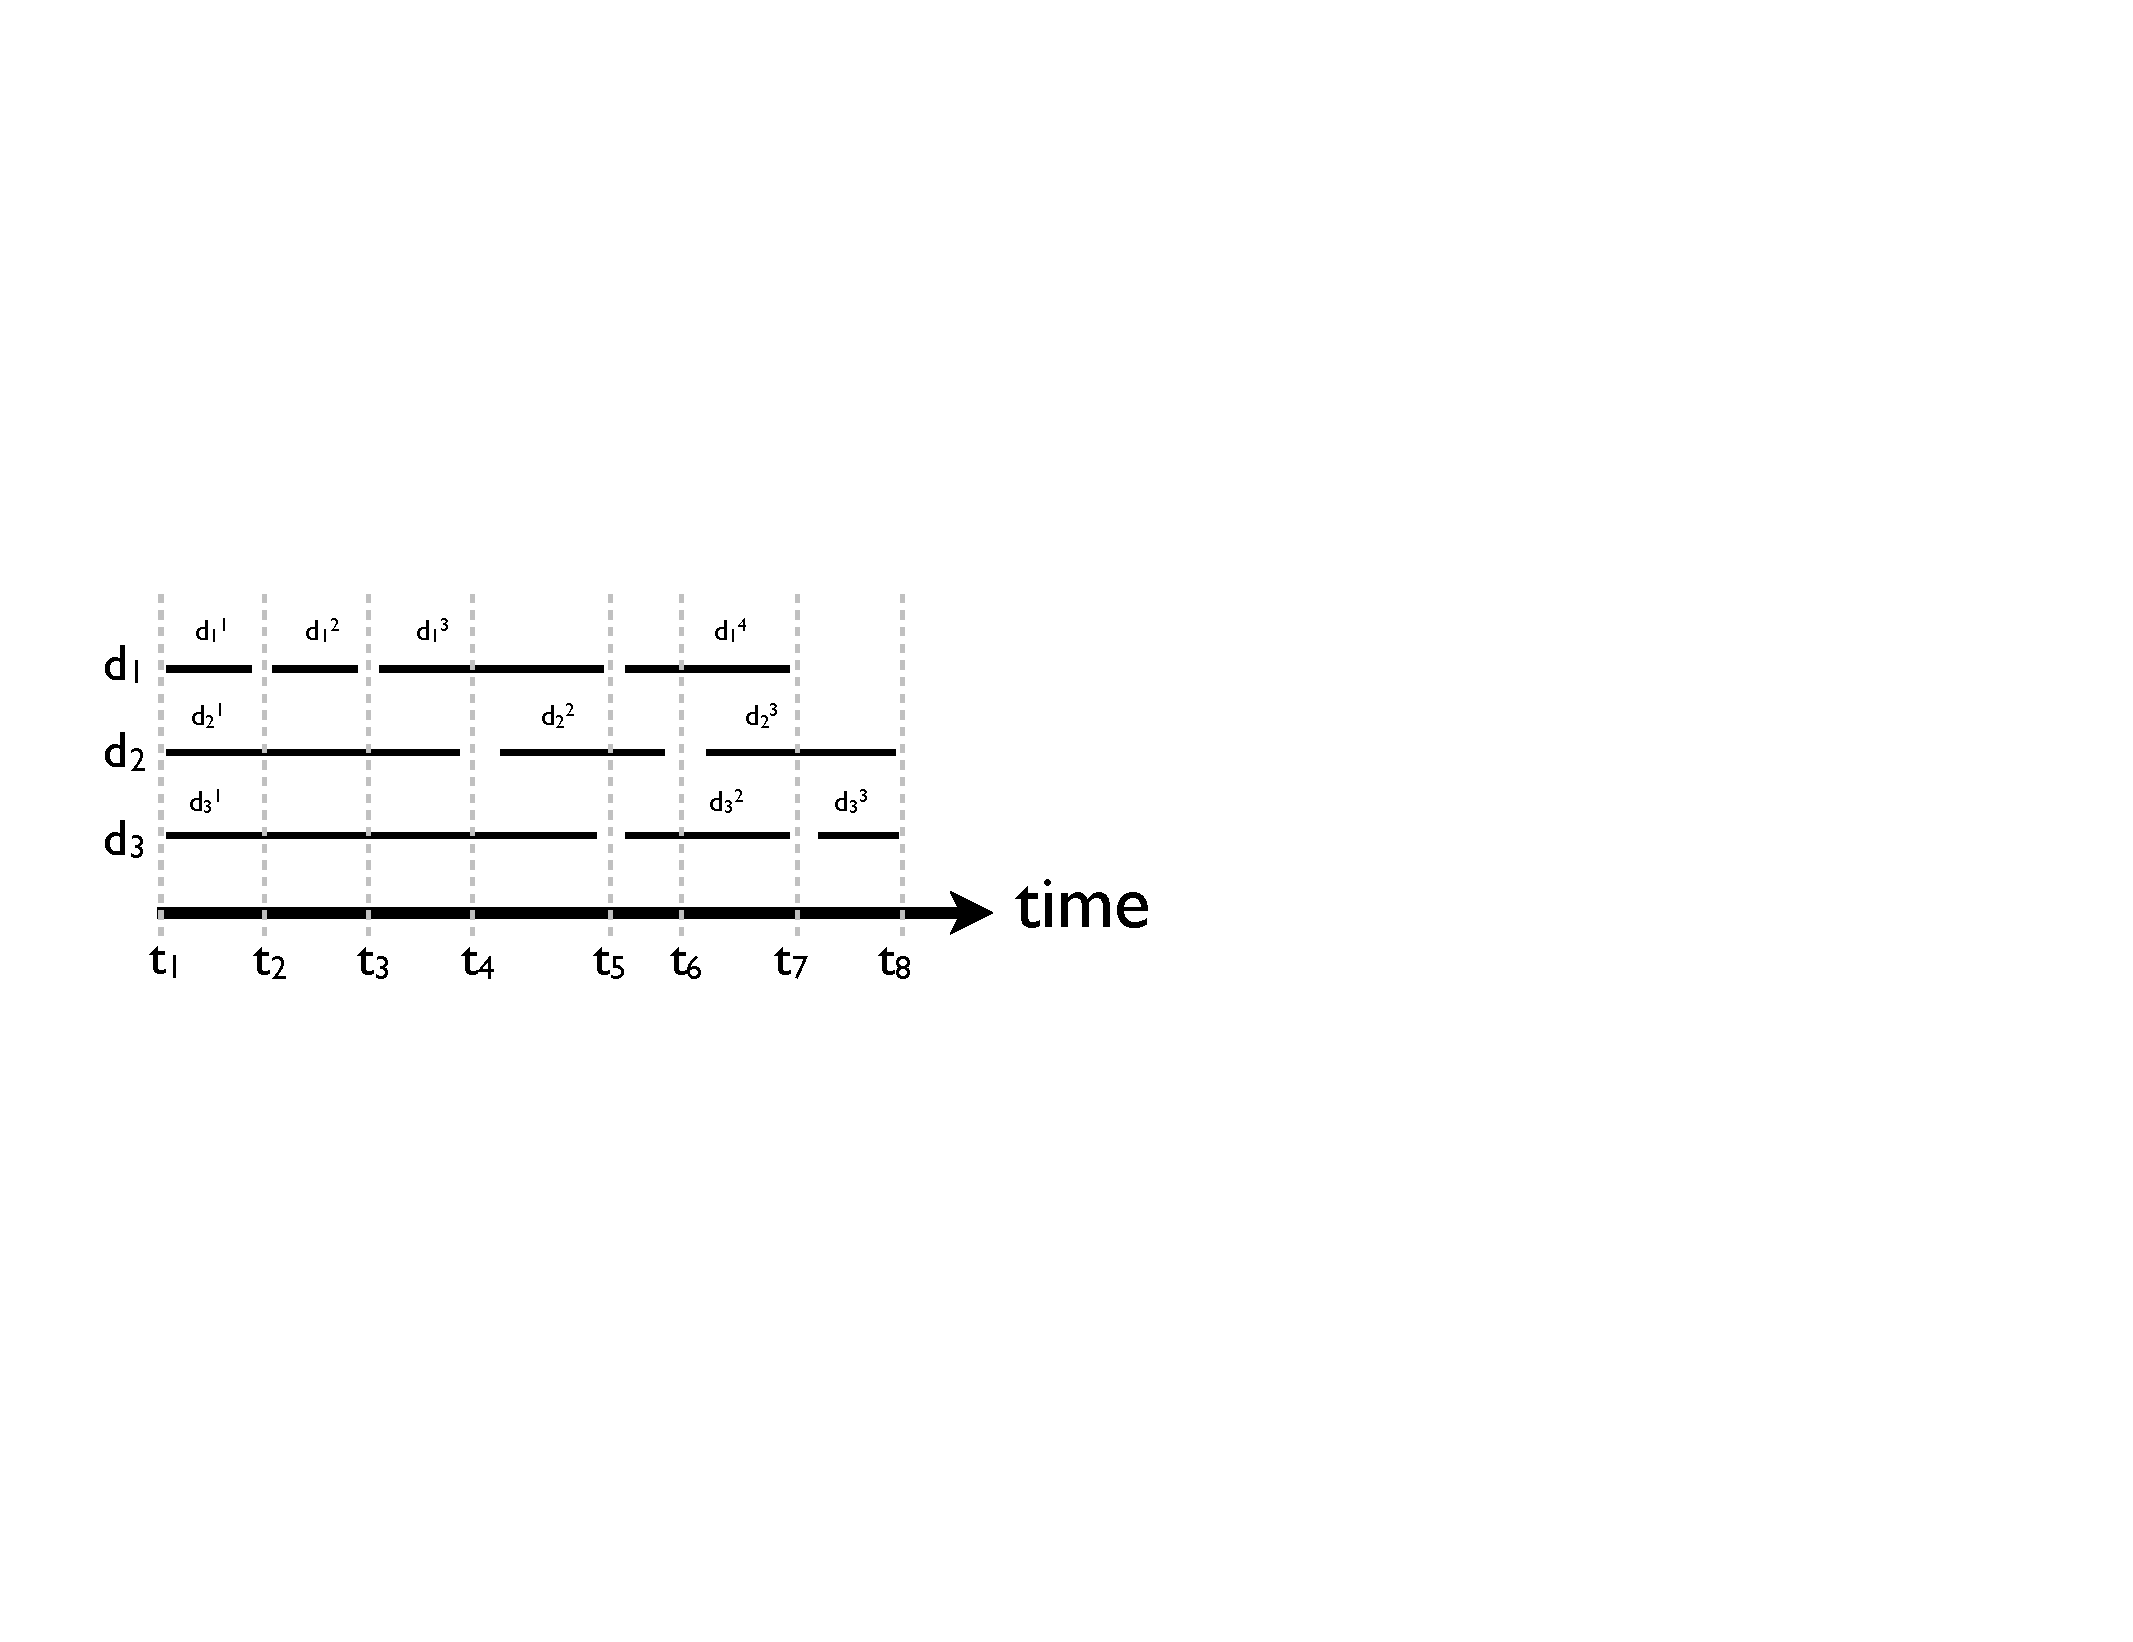
\includegraphics[width=0.7\columnwidth]{resources/popt.pdf}
  \caption{Partitioning a posting list} 
    \label{fig:part_strat}
\end{figure}

Following that, all partitions for the same term are merged and irrelevant postings, whose valid-time interval do not overlap with the query-time interval, are filtered out in the process. Note that identifying if a  postings is irrelevant in a partition is only possible once the partition is retrieved. If most of the postings in a partition are irrelevant then an entire partition must be wastefully read to determine a few relevant postings. An approach to reduce the cost of filtering out such postings, thus improving query performance, the granularity of partitioning can be reduced. As one extreme, called the \emph{performance-optimal} approach or $P_{opt}$, partition boundaries are placed at time-points that occur as boundaries of valid-time intervals as shown in the Figure~\ref{fig:part_strat}. Such a partitioning eliminates irrelevant postings in a partition.  

On the other hand, since each partition is associated with a time span, postings whose valid-time intervals overlap with multiple partitions are replicated in all of them. For instance, in Figure~\ref{fig:part_strat}, the version $d_3^1$ is replicated multiple times for the performance-optimal approach. Replication of postings in multiple partitions results in an index blowup thus making the performance-optimal approach infeasible in practice. The other extreme case, referred to as \emph{space-optimal} partitioning or $S_{opt}$, ensures that there is no index blowup by disallowing replication of postings. 

\paragraph{Partitioning Strategies} There is a natural trade-off between query performance and index-size blow and the above two approaches represent the two extremes of this. In practical situations the desired \emph{partitioning strategy} lies between these two strategies. To explore this middle ground two approaches of partitioning strategies are proposed - the \emph{performance guarantee} approach and the \emph{space bound} approach.  

In the performance guarantee approach a bounded loss of performance over $P_{opt}$ is tolerated. The reduction of performance, by the performance-guarantee approach, for a given query is measured by the excess of postings processed over $P_{opt}$. The performance reduction is bounded by a user specified parameter $\gamma$ and a partitioning is desired which adheres to this bound for all possible queries. The objective, under such a performance guarantee, is to minimize the overall index-size blowup. 

The space-bound approach is proposed for situations when storage space is at a premium and a bound is desired on the overall index size. Given a user specified index-size bound, $\kappa$, the objective here is to  minimize the reduction of performance relative to $P_{opt}$. The size bound on the entire index can be translated to a bound on the size of each posting list. The size bound for partitioning posting list for each term $v$ is given by $\kappa.|L_v|$. The space-bound approach also allows for a query distribution determining the probability of a term given a time-point $P(t)$. An optimization problem is formulated which intends to partition a posting list $L_v$ to minimize the expected query processing cost, given $\kappa$ and $P(t)$, while adhering to a space bound $\kappa.|L_v|$. We refer to these partitioning strategies as \emph{vertical partitioning} in the rest of the thesis.

  
\paragraph{Temporal Coalescing} 
 \begin{figure}[tb]
  \centering
    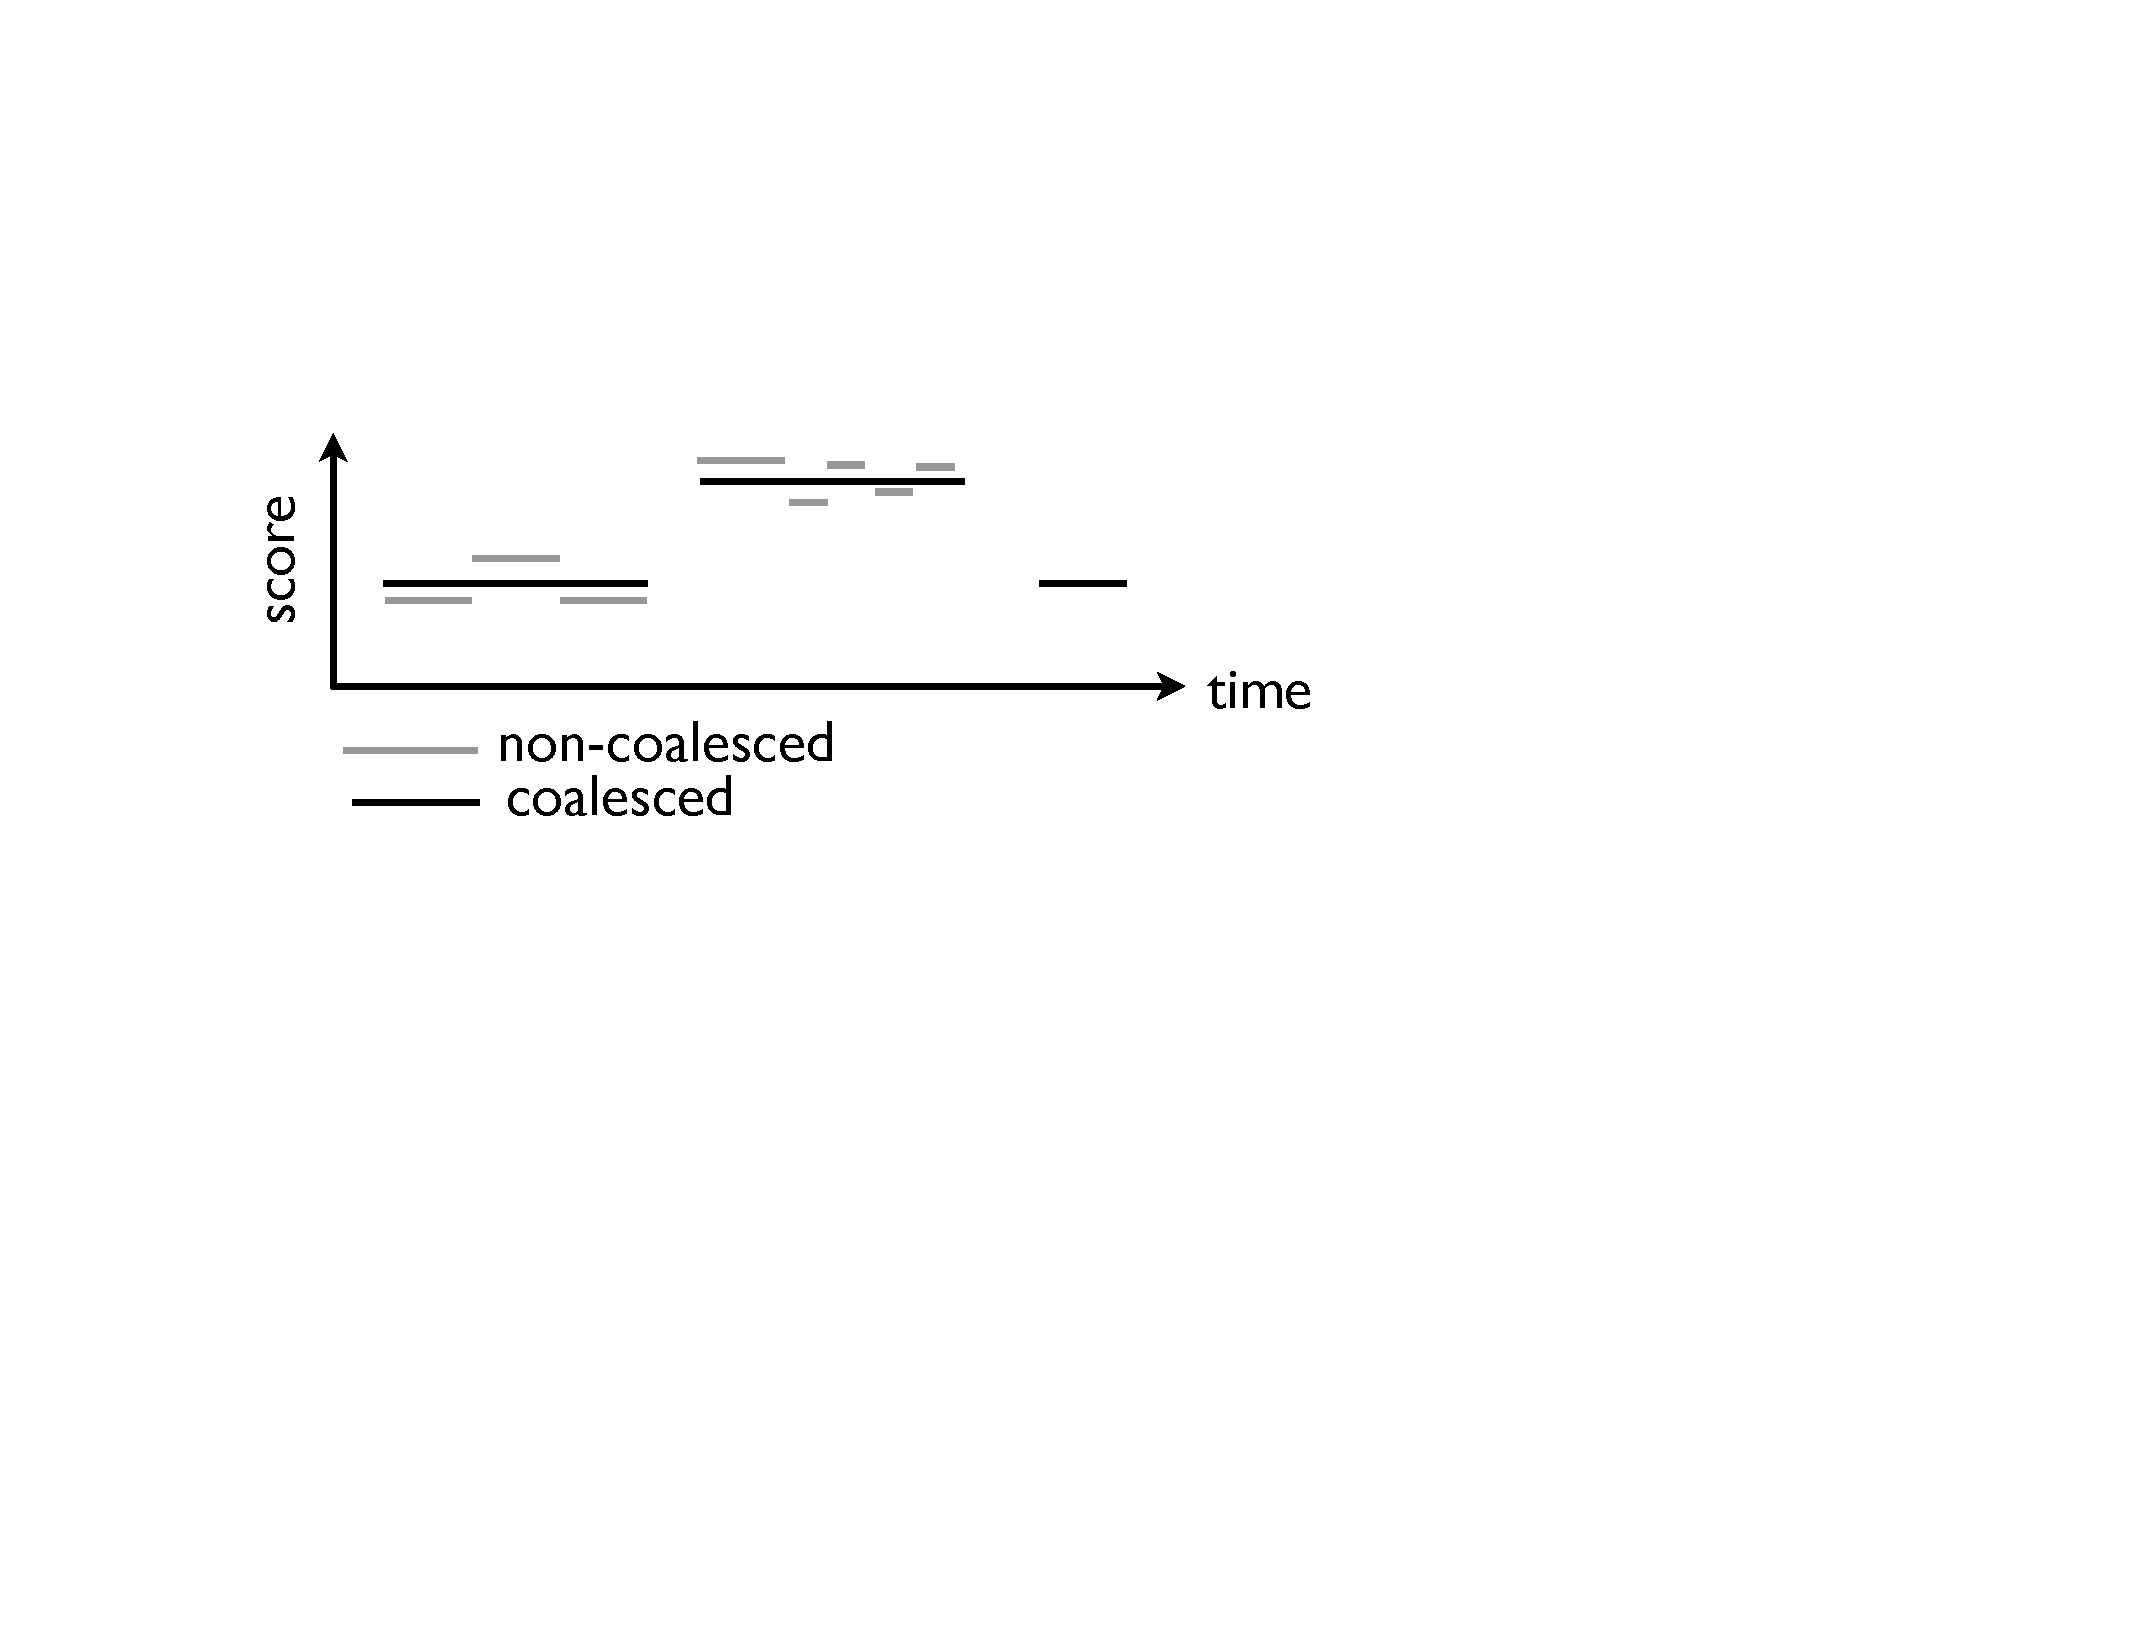
\includegraphics[width=0.7\columnwidth]{resources/coalescing.pdf}
  \caption{Temporal coalescing} 
    \label{fig:coalescing}
\end{figure}

Indexing all the versions is expensive in terms of storage costs. However, archives are characterized by a high degree of redundancy. Often times, changes to documents are minor resulting in a high overlap of text content between consecutive documents versions. Temporal coalescing techniques exploits this redundancy to substantially decrease the overall index size.

A na\"ive implementation of the posting list $L_v$ would create a posting for each document version term pair. To exploit the redundancy between consecutive versions temporal coalescing in conjugation with the time-travel index. Temporal coalescing methods aim to coalesce postings belonging to consecutive versions of the same documents when the information contained between them is not significantly different. The techniques are applied on a per-term basis. They also have different semantics for different types of payloads, i.e., boolean, scalar or positional.

For boolean payloads of the form $\langle d_i^k, valid(d_i^{k}) \rangle$, multiple postings for consecutively occurring versions can be replaced by a single posting. The single posting represents that the term was present in a document for a contiguous period of time encoded in the posting. 

For scalar payloads, scores of consecutive versions with low variance can be captured and coalesced into a single posting. Figure~\ref{fig:coalescing} illustrates that coalescing postings with small variation in scores results in reducing the number of postings, in this example, from 9 to 5. The degree of relaxation allowed is specified by the user and captured by the parameter $\eta$. This is formulated as an optimization problem. Given an input sequence of postings of the same document, ordered by their begin times, the objective is to generate a minimal number of coalesced postings adhering to the user specified relaxation. 

